\documentclass[a4paper,12pt]{article}

\usepackage{graphicx} % Required for inserting images
\usepackage{amsmath,amssymb,amsfonts}
\usepackage{subcaption}
% -----------------------
% Package Imports
% -----------------------

% Set page margins
\usepackage[a4paper, top=1in, bottom=0.8in, left=1.1in, right=0.8in]{geometry}

% Use Times New Roman font
\usepackage{times}

\usepackage{microtype}

\usepackage{array,booktabs,multirow,makecell}
\usepackage{bm}
\usepackage{siunitx}  % For proper unit handling


% Set page margins
\usepackage[a4paper, top=1in, bottom=0.8in, left=1.1in, right=0.8in]{geometry}


% Add page numbering
\pagestyle{plain}

% Enable graphics inclusion
\usepackage{graphicx}
\usepackage{float}
% Enable code listings
\usepackage{listings}
\usepackage{xcolor} % For customizing code colors
\setlength{\parindent}{0pt}
\usepackage{multirow}

\setlength{\parindent}{0pt}
\usepackage{titlesec} % To customize section font size
\titleformat{\section}
{\normalfont\fontsize{14}{16}\bfseries}{\thesection}{1em}{}

\titleformat{\subsection}
{\normalfont\fontsize{14}{16}\bfseries}{\thesubsection}{1em}{}

\begin{document}
	\section{Experiment No. 10}
	
	\section{Experiment Title }
	Starting a 3-Phase Induction Motor Using Star-Delta Starter Method.
	
	\section{Objective}
	
	The objectives of this lab are as follows:
	\begin{itemize}
		\item 	To understand the equivalent-circuit representation of a three-phase induction motor
		\item 	To determine the core losses and magnetizing branch parameters using the no-load test.
		
		\item  To find the stator and referred rotor resistance and leakage reactance using the locked-rotor
		test.
		
		
	\end{itemize}
	\section*{Theory}
	
	The Wye-Delta (Y-$\delta$) starter is a widely used method for starting three-phase induction motors, especially those with large power ratings. This starter temporarily connects the motor windings in a wye (Y) configuration during startup and then switches them to a delta ($\delta$) configuration for normal operation.
	
	This method is designed to reduce the inrush current and starting torque, both of which can be harmful to electrical and mechanical systems. The transition from Y to $\delta$ is typically automatic and takes place once the motor reaches a predefined speed (usually around 70--80\% of its rated speed).
		\section{Circuit Diagram}
	\begin{figure}[H]
		\centering
		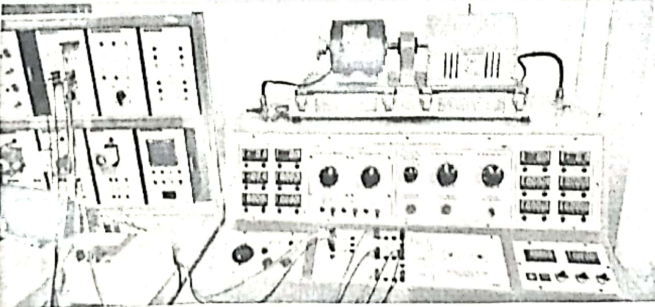
\includegraphics[width=0.6\linewidth]{Images/1}
		\caption{3 Phase Squirrel Cage Induction Motor}
	\end{figure}
	\subsection*{Purpose of the Wye-Delta Starter}
	
	\begin{enumerate}
		\item \textbf{Reduction of Starting Current:} At startup, the motor draws a significantly lower current due to the reduced voltage applied in the wye configuration. This helps avoid voltage drops and reduces stress on the electrical system.
		\item \textbf{Reduction of Starting Torque:} The starting torque is also reduced to one-third compared to direct-on-line (DOL) starting. This protects mechanical components from sudden shocks.
	\end{enumerate}
	
	\subsection*{Operation of the Wye-Delta Starter}
	
	\begin{enumerate}
		\item \textbf{Startup Phase (Wye Configuration):} Initially, the stator windings are connected in a wye configuration. In this setup, each phase of the motor receives only $\frac{1}{\sqrt{3}}$ (approximately 57.7\%) of the line voltage. As a result, both current and torque are reduced to about one-third of their full-load values.
		\item \textbf{Running Phase (Delta Configuration):} After the motor accelerates to about 70--80\% of its rated speed, the starter switches the winding connections from wye to delta. The motor then receives the full line voltage, allowing it to operate at its rated torque and speed.
	\end{enumerate}
	
	
	\section{Circuit Diagram}
	\begin{figure}[H]
		\centering
			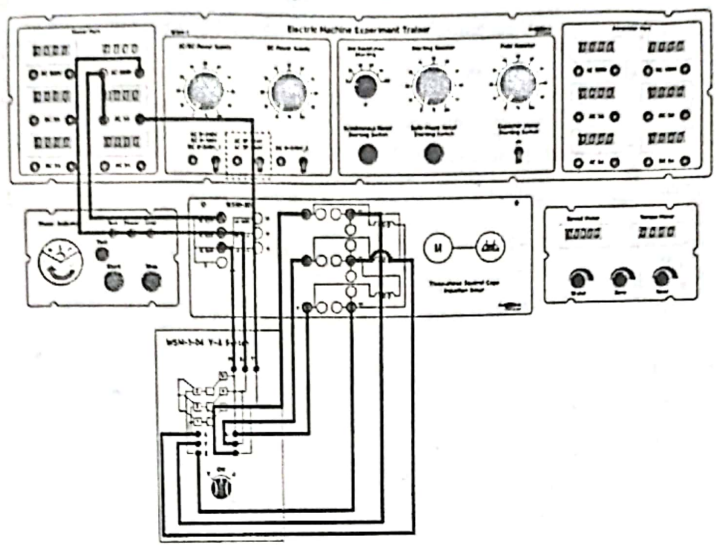
\includegraphics[width=0.6\linewidth]{Images/2}
		\caption{The connection diagram for the Y-$\Delta$ starter}
	\end{figure}
	

	
	\section{Required Apparatus}
	\begin{table}[H]
		\centering
		\caption{ List of Required Equipment}
		\begin{tabular}{|c|p{5.5cm}|p{6cm}|}
			\hline
			\textbf{SN} & \textbf{Equipment} & \textbf{Specification} \\
			\hline
			1 & 3-Phase Induction Motor & Output: 360W, Voltage: 220V, Current: 2.2A, Pole: 4, Speed: 1480 RPM \\
			\hline
			2 & AC Multimeter & $V_{\text{rms}}^{\text{max}} = 500\,\text{V}$, $I_{\text{max}} = 5\,\text{A}$ \\
			\hline
			3 & Electric Machine Equipment Trainer & – \\
			\hline
			4 & Star-Delta Switch Module & – \\
			\hline
		\end{tabular}
	\end{table}
	
	\section{Procedure}
	
	\begin{enumerate}
		\item Connect the motor and the starter according to the provided circuit diagram.
		\item Start the motor in star (Y) configuration and record the voltage, current, and speed.
		\item After the motor reaches the running condition, transition to delta ($\delta$) configuration.
		\item Record the voltage, current, and speed in delta mode.
		\item Compare the recorded data for both star and delta configurations.
	\end{enumerate}
	
	
	
	\section{Result}
	
	\begin{table}[H]
		\centering
			\caption{Data Table of Results}
		\begin{tabular}{|l|c|c|}
			\hline
			\textbf{Parameter} & \textbf{Star (Y)} & \textbf{Delta($\delta$)} \\
			\hline
			Voltage , (V) & 127.24(P-N) & 219.5 \\
			\hline
			Current,  (A) & 0.535 & 1.997  \\
			\hline
			Speed, (RPM) & 1499 & 1506 \\
			\hline
		\end{tabular}
	
	\end{table}
	
	
	\section{Discussion}
	
	The experimental data shows a significant difference in current between the star and delta configurations. In the star mode, the reduced voltage limits the current, thereby minimizing the initial inrush. Upon switching to the delta configuration, the motor receives the full line voltage, allowing it to generate its rated torque and speed. This confirms the practicality and efficiency of the star-delta starting method in managing startup stress in three-phase induction motors.
	
	\section{Conclusion}
	
	The star-delta starter is an effective method for reducing the initial inrush current during the startup of induction motors. It allows the motor to start under a reduced voltage and then transition to full operating conditions after reaching partial speed. This method provides both protection and performance, making it especially suitable for industrial applications where large motors are used.
	
	\section{Precautions}
	
	\begin{itemize}
		\item Do not exceed the motor’s rated load during operation.
		\item Avoid frequent transitions between star and delta configurations to prevent overheating.
		\item Ensure secure and accurate wiring before starting the experiment.
	\end{itemize}
	
	\section{Reference}
	
	Stephen J. Chapman, \textit{Electric Machinery Fundamentals}.
	
	
	
\end{document}
